\documentclass{beamer}
\usepackage{lsfolien}
\usepackage[english]{babel}

\myfootline{Sustainability, Environment, Management -- Summer Term
  2022}{Hans-Gert Gr\"abe}

\newcommand{\ueberschrift}[1]{\begin{center}\bf #1\end{center}}

\title{Systematic Innovation Methodology\vskip1em}

\subtitle{Research Seminar in the Module 10-202-2312\\ for Master Computer
  Science}

\author{Prof. Dr. Hans-Gert Gräbe\\
\url{http://www.informatik.uni-leipzig.de/~graebe}}

\date{April 2022}
\begin{document}

{\setbeamertemplate{footline}{}
\begin{frame}
  \titlepage
\end{frame}}

\begin{frame}{Omnipresence of the System Concept}

The concept of a \emph{system} plays a prominent role in computer science when
it comes to database systems, software systems, hardware systems, accounting
systems, access systems, etc.

In general, computer science is regarded by a majority as the \vskip1em
\begin{quote}
  "science of the \emph{systematic} representation, storage, processing and
  transmission of information, especially their automatic processing using
  digital computers" (German Wikipedia).
\end{quote}
Also certain relevant professions such as the \emph{system architect} are in
high esteem by IT users.
\end{frame}

\begin{frame}{Omnipresence of the System Concept}
However, the significance of the concept of system extends far beyond the
field of computer science -- it is fundamental for all engineering sciences
and as \emph{Systems Engineering} with the ISO/IEC/IEEE-15288 standard
"Systems and Software Engineering", it is also the subject of international
standardisation processes.

Even more, the concept of systems also plays an important role in the
description of complex natural and cultural processes -- for instance in the
concept of an \emph{ecosystem}.
\end{frame}

\begin{frame}{Omnipresence of the System Concept}
While classical TRIZ focuses strongly on instrumentally feasible engineering
solutions, Systems Engineering\vskip1em 
\begin{quote}
  is an interdisciplinary field of engineering and engineering management that
  focuses on how to design, integrate, and manage complex systems over their
  life cycles. At its core, systems engineering utilises systems thinking
  principles to organise this body of knowledge. The individual outcome of
  such efforts, an engineered system, can be defined as a combination of
  components that work in synergy to collectively perform a useful function.
  (English Wikipedia)
\end{quote}
\end{frame}

\begin{frame}{On the Notion of a System}

"Utilising systems thinking" refers to a system concept that describes
  \textbf{the purpose-oriented interaction of viable components in a delimited
    context for the provision of emergent functions}.

Such functions are not inherent to any of the components, but result from
their interaction within the context of a defined throughput of energy,
material and information, which is provided by an -- in systemic terms --
"external world".  See the lecture for more details.

Such approaches play a central role not only in the field of engineering, but
also in the field of business processes, systems and models. Systemic
approaches are linked to the concept of an \textbf{organisation} as a
socio-technical system. More about this in the handout \emph{Systems,
  Organisations, Management} in the github repo of this course.
\end{frame}

\begin{frame}{TRIZ and Systematic Innovation}
TRIZ is a Russian acronym and stands for \emph{Theory of Innovative Problem
  Solving}.

TRIZ is often perceived as a complex toolbox alone. In reality, it is a
problem-solving methodology with special focus on
\begin{itemize}
\item systemic modelling 
\item and solution of contradictions 
\item through conceptual integration into larger contexts
\item and systemic development according to dialectical principles.
\end{itemize}
This methodology can be applied to \emph{any planning approach}, including
non-technical areas such as Business and Management.
\end{frame}

\begin{frame}{TRIZ and Systematic Innovation}
  \begin{center}
    \includegraphics[width=\textwidth]{images/ProblemSolvingWithTRIZ.png}
    \vskip2em

    The general TRIZ solution pattern
  \end{center}
\end{frame}

\begin{frame}{TRIZ and Systematic Innovation}\small
  \begin{center}
  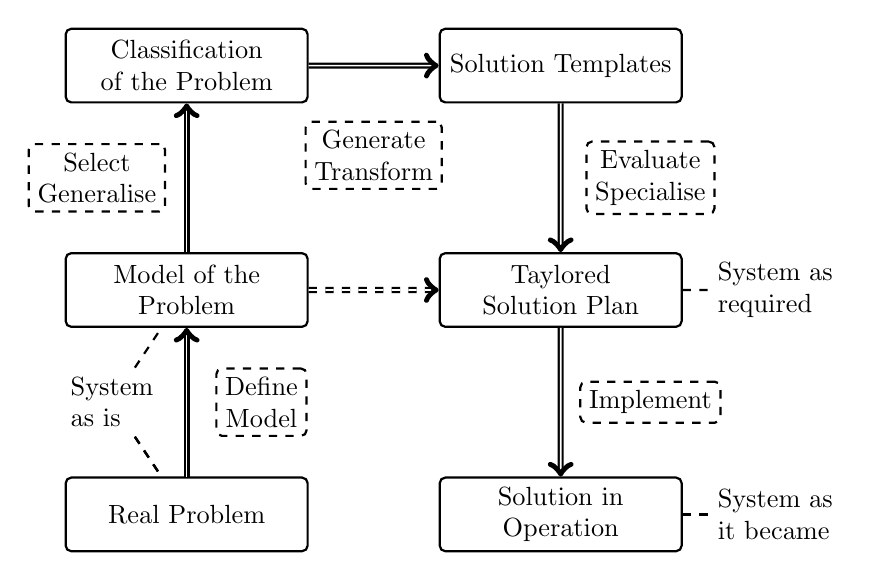
\begin{tikzpicture}[scale=.95,transform shape,
      textbox/.style={draw, text width=3cm, minimum height=2.8em,
        align=center},
      ovalbox/.style={draw, dashed, align=center},
      %>={Triangle[length=0pt 6,width=0pt 5]},
      rounded corners=2pt,line width=.8pt]

    \node[text width=1.1cm] at (-1,1.5) (A0) {System\\ as is};
    \node[textbox] at (0,0) (A1) {Real Problem};
    \node[ovalbox] at (1,1.5) {Define\\ Model}; 
    \node[textbox] at (0,3) (A2) {Model of the Problem};
    \node[ovalbox] at (-1.2,4.5) {Select\\ Generalise}; 
    \node[textbox] at (0,6) (A3) {Classification of the Problem};
    \node[ovalbox] at (2.5,4.8) {Generate\\ Transform}; 
    \node[textbox] at (5,6) (B3) {Solution Templates};
    \node[ovalbox] at (6.2,4.5) {Evaluate\\ Specialise}; 
    \node[textbox] at (5,3) (B2) {Taylored\\ Solution Plan};
    \node[ovalbox] at (6.2,1.5) {Implement}; 
    \node[textbox] at (5,0) (B1) {Solution in Operation};
    \node[text width=1.8cm] at (8,3) (C2) {System as\\ required};
    \node[text width=1.8cm] at (8,0) (C1) {System as\\ it became};

    \draw[-,dashed] (A0) -- (A1);
    \draw[-,dashed] (A0) -- (A2);
    \draw[-,dashed] (B1) -- (C1);
    \draw[-,dashed] (B2) -- (C2);
    \draw[-,dashed] (A0) -- (A1);
    \draw[-,dashed] (A0) -- (A1);
    
    \draw[double,->] (A1) -- (A2) ;
    \draw[double,->] (A2) -- (A3) ;
    \draw[double,->] (A3) -- (B3) ;
    \draw[double,->,dashed] (A2) -- (B2) ;
    \draw[double,->] (B3) -- (B2) ;
    \draw[double,->] (B2) -- (B1) ;
\end{tikzpicture}
\end{center}
\end{frame}

\begin{frame}{TRIZ and Systematic Innovation}
TRIZ methodologies are applied 
\begin{itemize}
\item to sharpen intended effects in functional modelling as an Ideal Final
  Result or Ideal Machine,
\item to identify negative (harmful) effects occurring during implementation, 
\item to localise such problems as contradictory behaviour in a delimitable
  "operational zone", 
\item and finally to resolve such contradictions by transforming a "system as
  it is" into a "system as required".
\end{itemize}
Such ideas and approaches can be transferred to non-technical areas in which
\emph{systemic thinking}, \emph{planning-based} cooperative action and thus
\emph{scientifically based practices} are established.
\end{frame}

\begin{frame}{TRIZ and Systematic Innovation}\small
In the last 20 years, in particular the field of \emph{organisational
  management} has developed in this direction.  This domain includes the
modelling of \emph{business processes} in smaller-scale internal BP landscapes
and more compact \emph{business models} in larger-scale inter-organisational
contexts.

TRIZ is an experience-based \emph{systematic} approach. \emph{Business TRIZ}
has been unfolding for about 20 years and actively promotes the transfer of
experience, embedded in other management cultures and approaches.

\begin{center}
  \includegraphics[width=.8\textwidth]{images/BusinessStages.png}
\end{center}
\end{frame}

\begin{frame}{TRIZ and Systematic Innovation}
In TRIZ as an \emph{application-oriented methodology}, "use cases" as
successful solutions to problems are an important driver for the further
theoretical development.

In this specificity, Business TRIZ meets with other management theories, which
also have to prove their effectiveness above all in \emph{practical}
applications.

For this purpose, specific consulting structures have emerged in the
management sector, in which such experiences \emph{converge} on an
inter-company level, are \emph{systematised}, \emph{consolidated} and
\emph{disseminated} via both consulting and training structures.

Business TRIZ is only one building block in this larger methodological
context.
\end{frame}

\begin{frame}{The Seminar}

\textbf{In the seminar}, we want to learn more about modelling approaches of
\emph{Business TRIZ} to business processes within a company, especially with
regard to contradictory requirement situations that cannot be solved by
compromises, but require a dialectical resolution in the sense of the TRIZ
methodology and the emergence of common conceptual and notational worlds.

The basis for student presentations are individual chapters from (Mann 2007).
Based on this material, particular Business TRIZ concepts are to be presented
in more detail in their relation to more general concepts of business
processes, systems and models.  See the file \texttt{Seminarplan.md} for
details.

\end{frame}

\begin{frame}{The Seminar}
The seminar is a \textbf{research seminar} in which we jointly explore
different aspects of Business TRIZ and related concepts.

With this seminar, we are approaching a topic that is new to us, which offers
the opportunity to participate in a joint academic explorative process on a
basis of equals.

This bears opportunities, but also challenges.  The students are expected to
actively participate in the seminar through seminar discussions, presentations
and last but not least by reading the relevant materials.

For the successful completion of the seminar, a topic has to be presented in
the seminar as discussion leader and a handout of 2--3 pages on the topic has
to be submitted in advance.
\end{frame}

\begin{frame}{The Seminar}

The seminar will be held weekly on Tuesdays 9-11 a.m. synchronously online.

Prior to each appointment participants have to study the assigned reading to
be in a position to discuss the problems in the seminar.

The seminar is moderated by a \emph{discussion leader}, who prepares a short
handout of 2--3 pages and makes it available to the participants in advance
\emph{before the seminar} (by Sunday evening).

The \textbf{primary source for the seminar plan} is the (actual version of
the) file \texttt{Seminarplan.md} in the github repository \emph{Seminar-S22}.
\end{frame}

\begin{frame}{Course Structure}
The course includes
\begin{itemize}
\item[$\bullet$] the lecture "Modelling Sustainable Systems and Semantic Web"
\item[$\bullet$] the seminar "Systematic Innovation Methodology"
\end{itemize}

You find more about the seminar in the Saxonian e-learning platform OPAL
\url{https://bildungsportal.sachsen.de/opal} in the course S22.BIS.SIM.  The
platform will be used for organisational purposes only.

You can access OPAL with the data of your studserv account.
\end{frame}

\begin{frame}{Course Structure}\vskip1em
In the \textbf{lecture} \emph{Modelling Sustainable Systems and Semantic Web}
(Thursdays 9-11 a.m.) important concepts such as\vspace{-1em}
\begin{itemize}
\item[$\bullet$] technology as a unity of socially available procedural
  knowledge, institutionalised procedures and private procedural skills,
\item[$\bullet$] sustainability requirements in systemic concepts,
\item[$\bullet$] digital changes and concepts of semantic web technologies,
\item[$\bullet$] concept and knowledge formation processes,
\item[$\bullet$] cooperative action, network economies and open culture
\end{itemize}\vspace{-1em}
are developed in more detail.

The lecture and the seminar are not directly related to each other, but
conceptual frameworks developed in the lecture will be heavily present in the
seminar.\vskip3em
\end{frame}

\begin{frame}{Organisational Matters}
The course can be taken for credit as Seminar Module 10-202-2312 (5 CP)
"Applied Computer Science".
\begin{itemize}
\item[$\bullet$] \textbf{Prerequisite for examination:} Successfully
  completed seminar.
\item[$\bullet$] \textbf{Examination:} Seminar paper.
\end{itemize}
\end{frame}

\begin{frame}{Data protection}

We follow an Open Culture approach not only theoretically but also practically
and make course materials publicly available. This also applies to the course
materials you have to produce (presentations, seminar papers) as well as to
(annotated) chat sessions of the seminar discussions, in which your names are
also mentioned. \textbf{We assume your consent to this procedure if you do not
  explicitly object}. The discussions themselves are not recorded.

\end{frame}

\begin{frame}{Summary}

\begin{itemize}
\item[$\bullet$] Lecture: Thursdays 9:15-10:45, SG 31-5
\item[$\bullet$] Continuously updated lecture plan and list of references in
  the \texttt{Lecture/README.md} file in the github Repo.  
\item[$\bullet$] Further (mainly organisational) information also in the forum
  of the OPAL course.
\item[$\bullet$] Seminar: Tuesdays 9:15-10:45, synchronous digital
\item[$\bullet$] Seminar online in the BBB room BIS.SIM,
  \url{https://meet.uni-leipzig.de/b/gra-w2c-fhz-qnp}
\end{itemize}
\begin{center}\LARGE\bf
  Questions ?
\end{center}

See also \texttt{2022-04-19/README.md} for additional information about the
goal of the course. 

\end{frame}

\end{document}
